%\pagenumbering{arabic}%start arabic pagination from 1 

\chapter{Praktická část}

V této kapitole je popsán software a postupy použité při implementaci a nasazení Vert.x aplikací.

\section{Návrh}

Hlavní částí aplikace budou tři verticly. Tyto verticly pak budou sloužit jako základ pro jeden z modulů.

\begin{description}
\item[main.js] stará se o spouštění celé aplikace v několika rolích
\item[editor.js] obsluha editoru
\item[database.js] obsluha událostí 
\end{description}

\subsection{Cíle aplikace}\label{sub:use_case}

\begin{itemize}
\item Přidání a odstranění myšlenkových map
\item Přidání a odstranění jednotlivých bodů v myšlenkové mapě
\item Přejmenování bodů v myšlenkové mapě
\end{itemize}

\begin{figure}
\begin{centering}
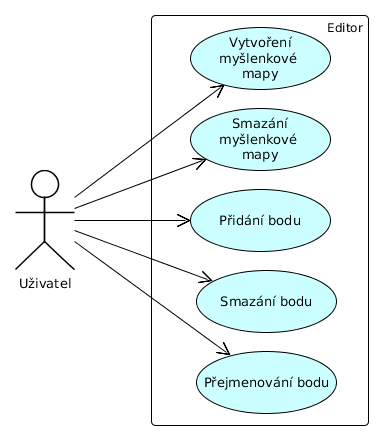
\includegraphics[scale=0.5]{obrazky/use_case}
\par\end{centering}
\caption{Případy užití\label{fig:use_case}}
\end{figure}

\FloatBarrier

\subsection{Architektura}

Jak je vidět na obrázku \ref{fig:architecture_real} klienti se budou připojovat přes jeden webový server, který bude spojený clusterem se serverem druhým. Na tomto serveru pak poběží samotná databáze. 

\begin{figure}
\begin{centering}
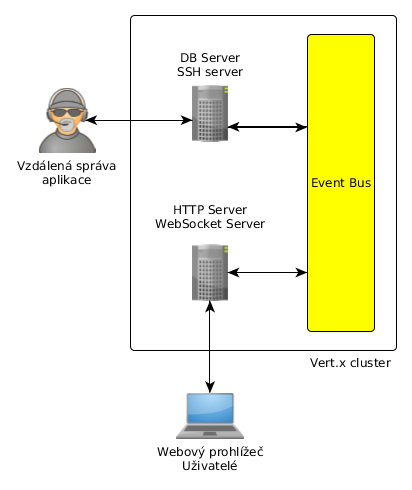
\includegraphics[scale=0.5]{obrazky/architecture_real}
\par\end{centering}
\caption{Architektura nasazené aplikace\label{fig:architecture_real}}
\end{figure}

\subsubsection{Adresářová struktura aplikace}

\begin{lstlisting}
main.js
editor.js
web
utils

vertx runmod io.majklk~mindmapeditor~0.0.1 -conf /srv/mindmap/conf/mindmajson -cluster-host 10.10.10.161 -ha
\end{lstlisting}



\section{Řídící verticle}

Vzhledem k tomu, že bude aplikace nasazená na více serverech ve více rolích bylo by potřeba napsat několik modulů podle zaměření, které tam startovat. To lze vyřešit napsáním ,,startéru", který dle konfigurace nastartuje příslušné moduly či verticly.

\begin{lstlisting}
JsonObject config = new JsonObject();
config.putString("foo", "wibble");
config.putBoolean("bar", false);
container.deployVerticle("foo.ChildVerticle", config);
\end{lstlisting}

Spuštění verticle z příkazové řádky
\begin{lstlisting}
vertx run foo.js -conf myconf.json
\end{lstlisting}

\section{Integrace s databází MongoDB}

Vzhledem k jednoduchosti aplikace nebyl vytvořen diagram tříd. V aplikaci budou pouze dva modely a to mapa a její potomek, který se od mapy liší pouze tím, že má místo globálního unikátního identifikátoru pouze unikátní identifikátor v rámci jedné mapy.

\begin{description}
\item[\_id] unikátní identifikátor\footnote{podtržítkem se běžně označující neměnné proměnné}
\item[name] název samotné mapy
\item[children] potomci
\end{description}

\begin{lstlisting}
{
	"_id": "1234-6545-5612-3456",
	"name": "Živočichové",
	"children": [
		{
			"key": "1",
			"name": "Obratolvci",
			"children": [
				{
					"key": "2",
					"name": "Ryby"
				},
				{
					"key": "3",
					"name": "Plazi"
				}
			]
		},
		{
			"key": "4",
			"name": "Bezobratlí"
		}
	]
}
\end{lstlisting}

\section{Komunikace v reálném čase}\label{sec:realTimeCommunication}

Po načtení myšlenkové mapy přichází na řadu aspekty komunikace v reálném čase. V rámci editoru myšlenkových map budou implementovány tři základní operace.
\begin{itemize}
\item Přidání objektu do myšlenkové mapy
\item Odstranění objektu z myšlenkové mapy
\item Přejmenování objektu v myšlenkové mapě
\end{itemize}
V tradiční webové aplikaci by to znamenalo implementaci těchto metod typem požadavek-odpověď jako operací konkrétní API. Při přidání objektu by se zavolala API a nazpět by přišla odpověď zda-li byla akce úspěšná. Pokud bychom však chtěli mít editor, který by propagoval změny ke všem, kdo mají myšlenkovou mapu otevřenou museli bychom znát přihlášené uživatele, kterým by server poslal notifikaci o změně. Mnohem jednoduší cesta je rozdělení požadavku a odpovědi do dvou částí což odpovídá návrhovému vzoru Command. V takovém případě při otevření webového prohlížeče s danou myšlenkovou mapou dojde k zaregistrování klienta na určitou adresu. V případě jakékoli změny, kterou provede jiný uživatel nebo kdokoliv jiný, dojde k odeslání události všem zaregistrovaným klientům okamžitě v době vykonání události. Tuto situaci lze vidět na obrázku \ref{fig:realtime_communication}. V případě, kdy u uživatele dojde k vyvolání akce, ostatním uživatelům bude zaslána událost, která s sebou nese všechny informace o změně. Všem klientům zaregistrovaným na stejnou adresu přijde stejná událost. Tento typ zasílání zpráv je znám jako návrhový vzor Publish/Subscribe.

\begin{figure}
\begin{centering}
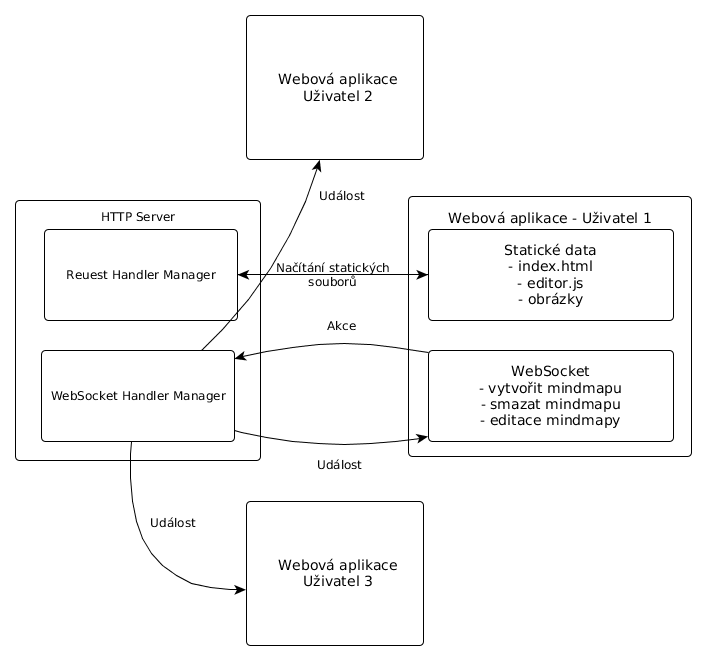
\includegraphics[width	=1\textwidth]{obrazky/realtime_communication}
\par\end{centering}
\caption{Komunikace v reálném čase\label{fig:realtime_communication}}
\end{figure}

\subsection{Akce}

Když bude uživatel chtít změnit myšlenkovou mapu (přidat objekt, odebrat objekt nebo přejmenovat objekt), vyšle akci na server. Tato akce bude poslána přes přemostěný event bus, který byl představen v kapitole \ref{sub:eventBus}. Na straně serveru je pak verticle, který má zaregistrovány metody na příchozí akce. Samotná akce nemá žádnou návratovou hodnotu, pokud tak dojde k chybě nedojde k vyslání události, která s sebou nese změny myšlenkové mapy.

\subsection{Události}

Pokud uživatel otevře webový prohlížeč s konkrétní myšlenkovou mapou, dojde tak k přihlášení odběru událostí nad touto myšlenkovou mapou. Pokud ji někdo změní tento uživatel dostane stejnou událost s informací o změně jako každý jiný uživatel přihlášený k odběru událostí.
Na straně klienta tak budou implementovány metody, které budou mít definované chování pro každou z definovaných událostí: přidání, odebrání a přejmenování objektu v myšlenkové mapě.

\section{Polyglot vývoj a moduly}\label{sec:praktickyModuly}

Každý modul ve Vert.x platformě musí spl

 deskriptor\emph{toto je poze základní výčet parametrů všechny lze nalézt v dokumentaci Vert.x}

Jmenná konvence pro jména modulů \emph{com.mycompany~my-mod~1.0}.

\begin{lstlisting}
{
  "main": "EchoServer.java",
  "worker": true,
  "includes": "io.vertx~some-module~1.1",
  "auto-redeploy": true
}
\end{lstlisting}

\begin{figure}
\begin{centering}
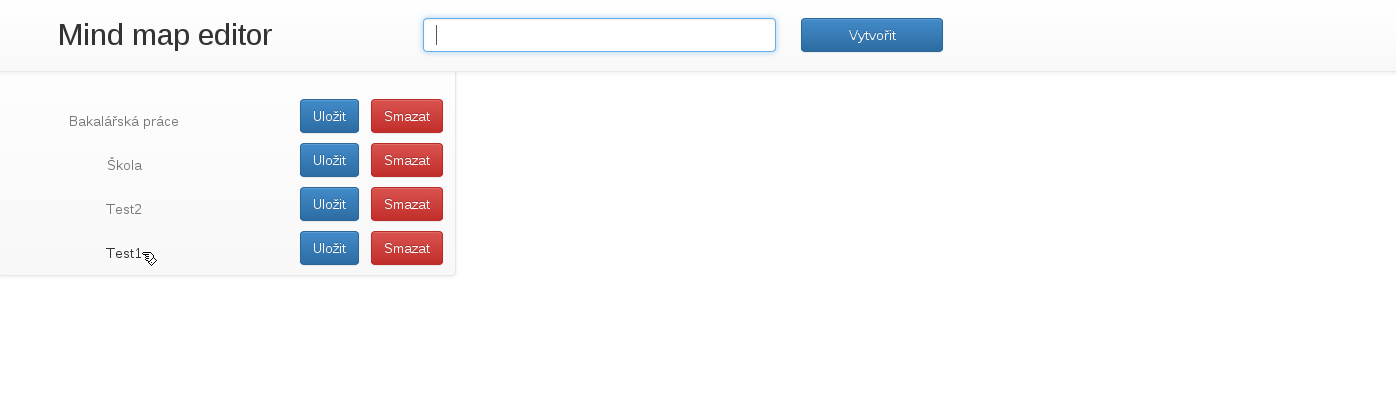
\includegraphics[width	=1\textwidth]{obrazky/mindmap1}
\par\end{centering}
\caption{Webová aplikace\label{fig:midnmap1}}
\end{figure}

\begin{figure}
\begin{centering}
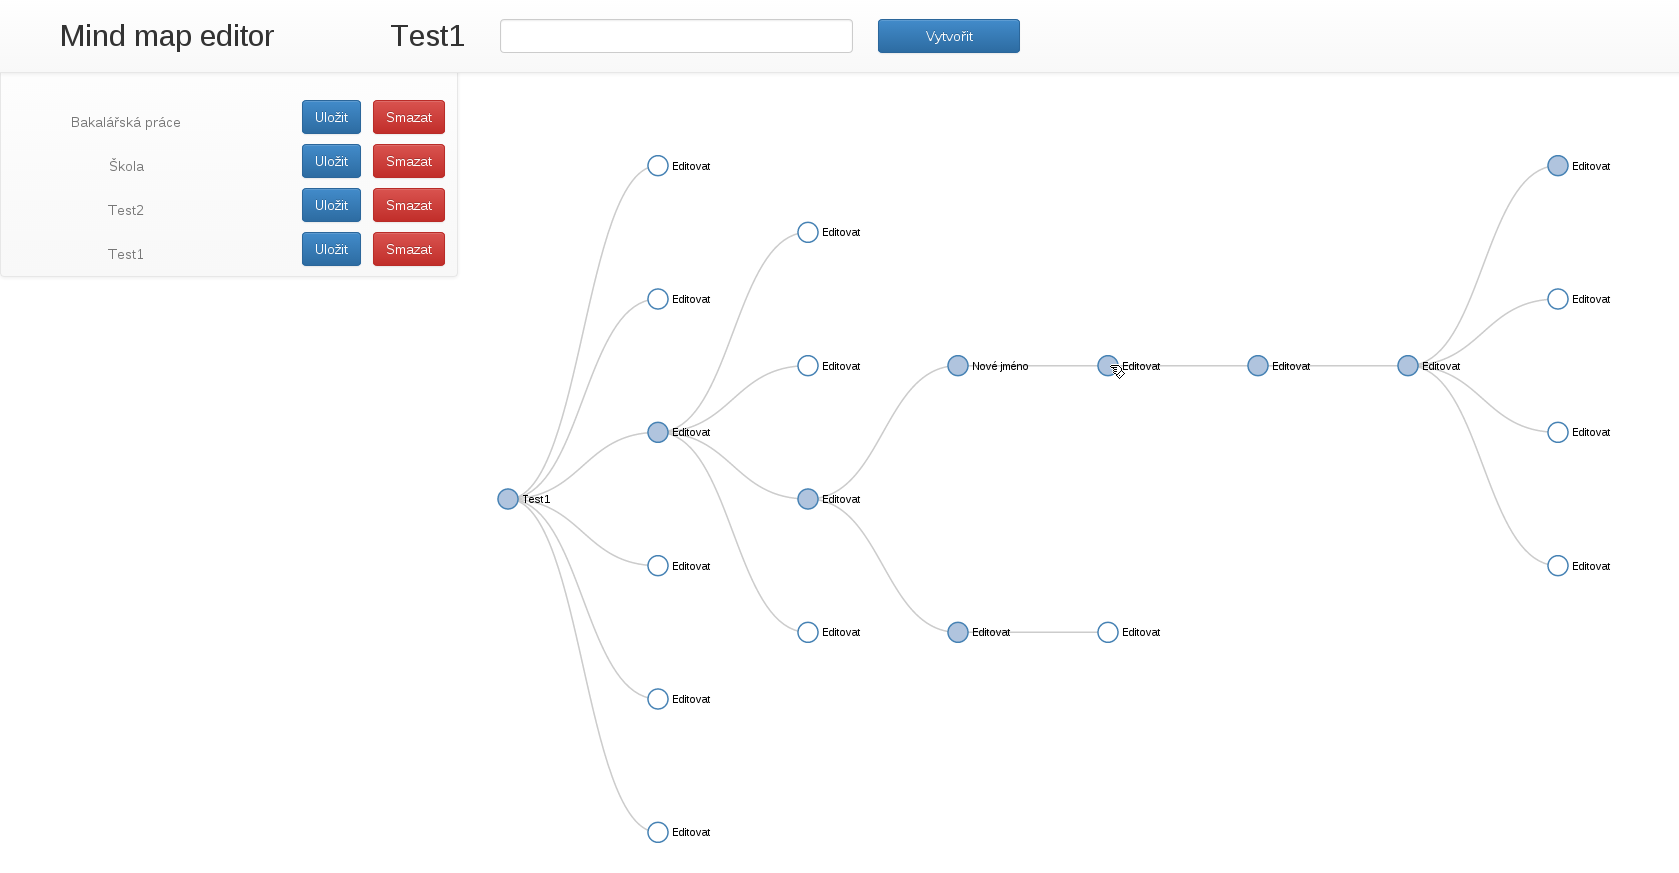
\includegraphics[width	=1\textwidth]{obrazky/mindmap2}
\par\end{centering}
\caption{Webová aplikace - otevření myšlenkové mapy\label{fig:midnmap2}}
\end{figure}

\begin{figure}
\begin{centering}
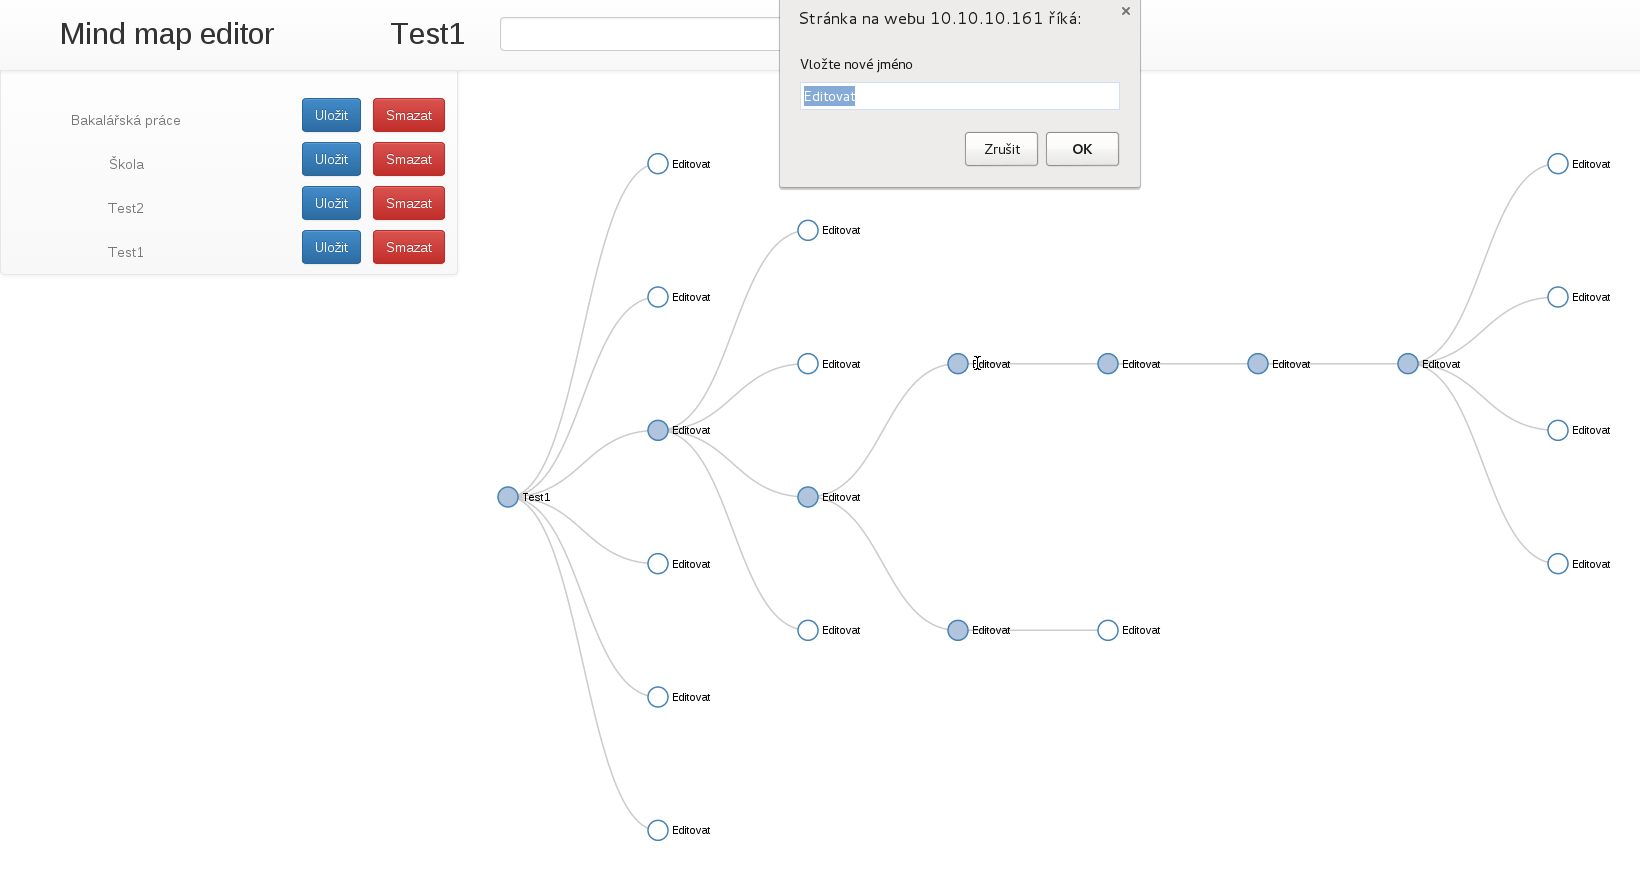
\includegraphics[width	=1\textwidth]{obrazky/mindmap3}
\par\end{centering}
\caption{Webová aplikace - akce - editace\label{fig:midnmap3}}
\end{figure}

Parametr \emph{auto-redeploy} mluví sám za sebe.

Jak bylo řečeno v \ref{sub:hybrid} Vert.x instance má dvě sady vláken. Parametrem \emph{worker} v deskriptoru modulu, lze říci Vert.x jádru aby spustil modul v \emph{background worker poolu}. 

Spuštění modulu programově v jazyce Java
\begin{lstlisting}
container.deployModule("io.vertx~mod-mailer~2.0.0-beta1", JSONconfig);
\end{lstlisting}

Spuštění modulu z příkazové řádky
\begin{lstlisting}
vertx runmod com.mycompany~my-mod~1.0 -conf config.json
\end{lstlisting}

moduly vice jazyku

\section{Základní služby}

Jádrem serveru je operační systém Ubuntu\cite{ubuntu} 14.04 LTS\footnote{dlouhodobá podpora} Server Edition s kódovým označením 
Trusty Tahr. Je to osvědčený systém, který bude mít podporu do roku 2019. Systém má aplikaci pro správu softwarových balíků 
aptitude. Všechny aplikace kromě samotného Vert.x šli hravě nainstalovat.

\subsection{Java}

Jako hlavní přísadou celého prostředí je otevřená implementace Java Platform, knihovna OpenJDK ve verzi 7.

\subsection{Vert.x}

Jediná služba, která se zatím nenachází jako systémový balíček je samotný Vert.x. Pro jeho instalaci je nutné stáhnout distribuci ze stránek platformy. Tento archiv potom rozbalit do požadované lokace. Následně stačí v závislosti na konkrétním systému přidat soubor \emph{vertx/bin/vertx} do systémové proměnné \emph{PATH}. Následně by měla být funkční interakce s platformou skrz příkazovou řádku. Příklad proměnné \emph{PATH} lze vidět v kapitole \ref{sub:service}. Správné nastavení lze otestovat napsáním \emph{vertx} do příkazové řádky. Správný výstup jsou pak pomocné informace pro komunikaci s platformou tzv. help.

\subsection{Databázový server}

Pro ukládání myšlenkových map je použita NoSQl databáze MongoDB ve verzi 2.6. MongoDb má za sebou více než pět let vývoje a několik obřích investicí. Vzhledem k tomu, že již existuje Vert.x modul pro pohodlnou spolupráci s touto databází byla vybrána pravě tato NoSQL databáze.

\subsection{Nasazení produkční služby}\label{sub:service}

V současné verzi(2.1.2) Vert.x nepodporuje běh v režimu daemon\footnote{je program, který běží v pozadí, čeká na události, které nastanou, reaguje na ně a poskytuje služby.}. Nasazení v režimu daemon je však nutnost pro běh v produkčním prostředí. Pro běh aplikace MindMap editoru byla využita systémová služba Supervisord\footnote{supervisord.org}, která běží jako linuxový daemon a stará se o běh aplikace, v případě pádu se ji pokusí znovu nasadit. Samotná konfigurace služby pro běh v Supervisordu pak obsahuje základní parametry. V verzi 3.0 je však plánovaná funkce běhu v režimu daemona a nebude tak tato berlička potřeba.

\begin{lstlisting}
[program:vertx_mindmap_editor]
directory=/srv/mindmap/app
environment=PATH="/srv/vert.x-2.1RC3/bin/vertx"
environment=JAVA_HOME="/usr/lib/jvm/java-7-openjdk-amd64/"
command=vertx runmod io.majklk~mindmapeditor~0.0.1 -conf /srv/mindmap/conf/allinone.json
user=root
autostart=true
autorestart=true
redirect_stderr=true
stdout_logfile=/srv/mindmap/app/app.log
stderr_logfile=/srv/mindmap/app/error.log
startsecs=10
stopwaitsecs=600
\end{lstlisting}


\section{Horizontální a vertikální škálování}\label{sub:Scaling}

sadsadasdds
\begin{figure}
\begin{centering}
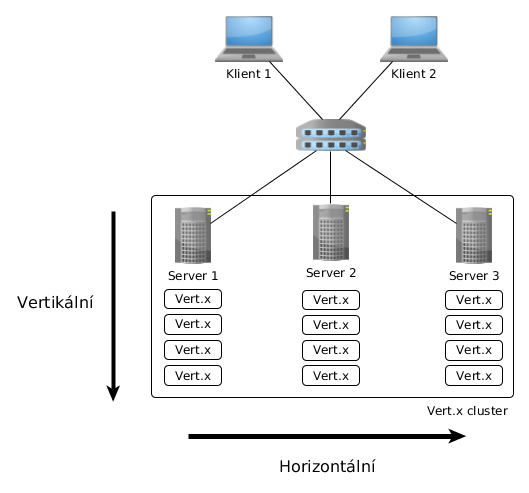
\includegraphics[scale=0.5]{obrazky/scaling_example}
\par\end{centering}
\caption{Horizontální a vertikální škálování\label{fig:scaling_example}}
\end{figure}

\FloatBarrier

scaling

možnosti škálování a HA

Server 1
\begin{lstlisting}
command=vertx runmod io.majklk~mindmapeditor~0.0.1 -conf /srv/mindmap/conf/webserver.json -cluster-host 10.10.10.162 -ha
\end{lstlisting}

Server 2
\begin{lstlisting}
command=vertx runmod io.majklk~mindmapeditor~0.0.1 -conf /srv/mindmap/conf/dbserver.json -cluster-host 10.10.10.162 -ha
\end{lstlisting}

\subsection{Vertikální}

Samotné vertikální škálování lze efektivně řešit na aplikační úrovni. Jak již bylo zmíněno v kapitole \ref{sub:multireactor} voláním \emph{Runtime.getRuntime().availableProcessors()} lze získat počet procesorových jader a s tím dále pracovat. Upravením předchozích příkazů však docílíme shodného výsledku.

\begin{lstlisting}
command=vertx runmod io.majklk~mindmapeditor~0.0.1 -instances 4 -conf /srv/mindmap/conf/dbserver.json -cluster-host 10.10.10.162 -ha
\end{lstlisting}

\subsection{Interakce s Vert.x}\label{sub:interaction}

Díky modulu CrasHub Shell\footnote{https://github.com/crashub/mod-shell} se lze protokolem SSH\footnote{Secure Shell} přihlásit přímo do Vert.x. Modul pak nabízí možnost interakce s jednotlivými komponentami samotného Vert.x. Lze například posílat zprávy přes Event Bus nebo nasazovat nové moduly za běhu celé aplikace. Samotný modul pak nabízí jednoduchou možnost přidání vlastním příkazů. Na obrázku je pak vidět přehledová obrazovka. Na obrázku \ref{fig:real_interaction} pak je hlavní přehledová stránka na které lze vidět činnost, vytížení a status všech vláken v celém clusteru. Dostupné jsou také informace o velikosti zásobníku, paměti či verze Javy. 

\begin{figure}
\begin{centering}
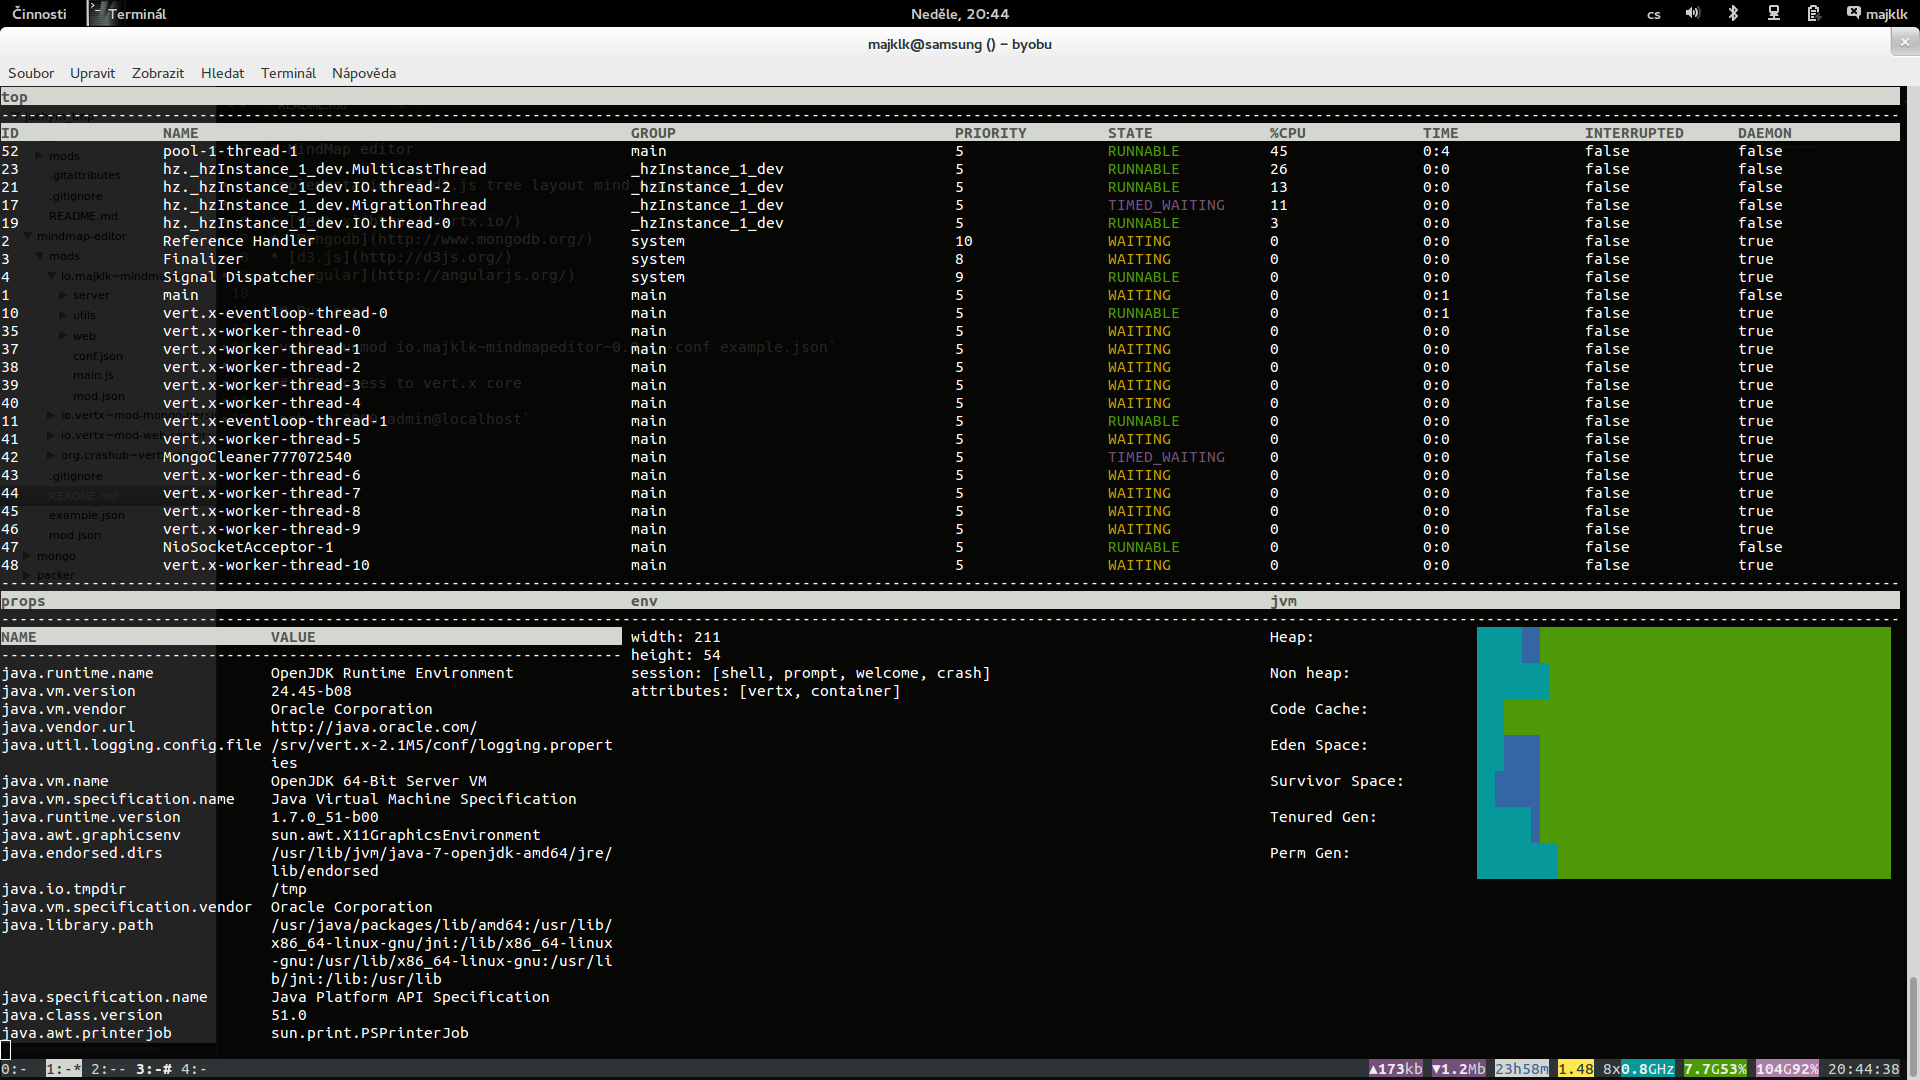
\includegraphics[scale=0.21]{obrazky/real_interaction}
\par\end{centering}
\caption{Modul CrasHub Shell\label{fig:real_interaction}}
\end{figure}

\subsection{Vert.x v clusteru}\label{sub:praktCluster}

Pro zajištění bezpečnosti databázového serveru, kde běží také služba pro vzdálený přístup k Vert.x instanci bude aplikace nasazena v clusteru. Webový server(HTTP Server) na obrázku \ref{fig:architecture_real} je připojen do dvou sítí.

\begin{description}
\item[Internet] pouze webový server
\item[Síť clusteru] všechny servery
\end{description}

Pro maximální bezpečnost budou na webovém serveru otevřeny pouze porty 80 a 443. Na druhém serveru pak poběží samotná databáze a druhá část aplikace, která v sobě bude zahrnovat modul zajištující komunikaci s databází a modul pro vzdálenou správu Vert.x instancí, který byl představen v kapitole \ref{sub:interaction}.

\section{Vysoká dostupnost}

Pro zajištění vysoké dostupnosti klíčových prvků aplikace, je potřeba upravit architekturu clusteru. Před webový server je postavená HA proxy\footnote{služba zajištující vyrovnávání zatížení}, která při úpadku jednoho z webových serverů přesměruje komunikaci na server druhý. Vert.x cluster je pak rozdělený na dvě HA skupiny(obr.\ref{fig:architecture_ideal}), které se liší svým zaměřením. První dva servery slouží jako webové a jsou napojeny na HA proxy. Další dva pak slouží pro komunikaci s databází, která na nich ležet nemusí.

\begin{figure}
\begin{centering}
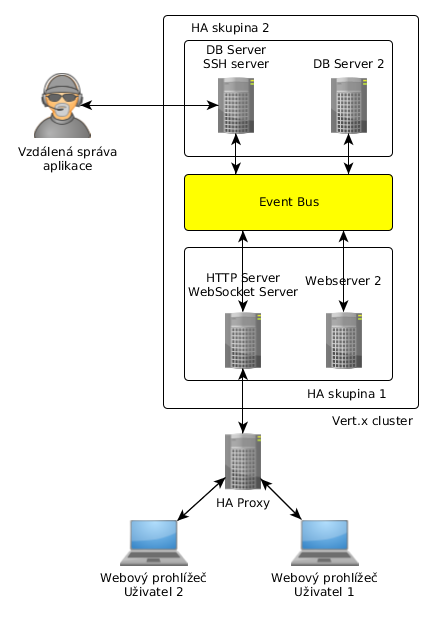
\includegraphics[scale=0.5]{obrazky/architecture_ideal}
\par\end{centering}
\caption{Ideální architekutra nasazení aplikace\label{fig:architecture_ideal}}
\end{figure}
